% --------------------------------------
% Document Class
% --------------------------------------
\documentclass[a4paper,11pt]{article}
% --------------------------------------



% --------------------------------------
% Use Package
% --------------------------------------


\usepackage[francais]{babel}
%\usepackage{ucs}
\usepackage[utf8]{inputenc}
\usepackage[T1]{fontenc}

\usepackage{makeidx}
\usepackage{color}
\usepackage{graphicx}
\usepackage{float}
\usepackage[hidelinks]{hyperref} 
\usepackage{geometry}
%\usepackage{lastpage}
%\usepackage{marginnote}
\usepackage{fancyhdr}
%\usepackage{titlesec}
%\usepackage{framed}
\usepackage{amsmath}
\usepackage{empheq}
\usepackage{array}
\usepackage{multicol}
%\usepackage{adjustbox}

% insert code
\usepackage{listings}

% define our color
\usepackage{xcolor}

% code color
\definecolor{ligthyellow}{RGB}{250,247,220}
\definecolor{darkblue}{RGB}{5,10,85}
\definecolor{ligthblue}{RGB}{1,147,128}
\definecolor{darkgreen}{RGB}{8,120,51}
\definecolor{darkred}{RGB}{160,0,0}

% other color
\definecolor{ivi}{RGB}{141,107,185}


\lstset{
    language=Scilab,
    captionpos=b,
    extendedchars=true,
    frame=lines,
    numbers=left,
    numberstyle=\tiny,
    numbersep=5pt,
    keepspaces=true,
    breaklines=true,
    showspaces=false,
    showstringspaces=false,
    breakatwhitespace=false,
    stepnumber=1,
    showtabs=false,
    tabsize=3,
    basicstyle=\small\ttfamily,
    backgroundcolor=\color{ligthyellow},
    keywordstyle=\color{ligthblue},
    morekeywords={include, printf, uchar},
    identifierstyle=\color{darkblue},
    commentstyle=\color{darkgreen},
    stringstyle=\color{darkred},
}


% --------------------------------------



% --------------------------------------
% Page setting
% --------------------------------------
%\pagestyle{empty}
\setlength{\headheight}{15pt}

\setcounter{secnumdepth}{3}
\setcounter{tocdepth}{2}

\makeatletter
\@addtoreset{chapter}{part}
\makeatother 

\hypersetup{         % parametrage des hyperliens
  colorlinks=true,      % colorise les liens
  breaklinks=true,      % permet les retours à la ligne pour les liens trop longs
  urlcolor= blue,       % couleur des hyperliens
  linkcolor= black,     % couleur des liens internes aux documents (index, figures, tableaux, equations,...)
  citecolor= green      % couleur des liens vers les references bibliographiques
}

% --------------------------------------

% --------------------------------------
% Information
% --------------------------------------
\title{Compte-rendu TP3 TI : Images discrètes}
\author{Elliot VANEGUE et Gaëtan DEFLANDRE}
% --------------------------------------

\definecolor{myColor}{rgb}{0.5, 0.1, 0.75}

% --------------------------------------
% Begin content
% --------------------------------------
\begin{document}

% Set language to english
  \selectlanguage{francais}

  % Start the page counting
  \pagenumbering{arabic}

  \maketitle
  
  \mbox{}
  \newpage
  \clearpage
  
  \section*{Introduction}
  Ce TP a pour objectif de détailler la composition d'une image couleur afin de pouvoir 
  effectuer des traitements de rééchantillonnement dessus. Nous allons donc chercher à sur-échantilloner et à 
  sous-échantillonner une image afin de comprendre les limites de ce procédé.
  
  \section{Composantes d'une image couleur}
  Nous allons d'abord voir comment manipulé les composantes d'une image couleur à partir de l'image de calibrage
  de couleur fournit dans le TP. On peut voir que la taille de la variable contenant l'image est de 1 440 000,
  qui correspond à $<largeur> * <hauteur> * <nombre de canaux>$.\\
  
  Pour récupérer la composante d'une couleur en image de gris, il suffit de récupérer le vecteur d'une des composantes
  et de l'afficher seul. Nous avons ainsi une matrice avec les valeurs de rouge et vu que nous ne gardons qu'une matrice,
  l'image se transforme en dégradé de gris.\\
  
  \begin{figure}[H]
    \center
    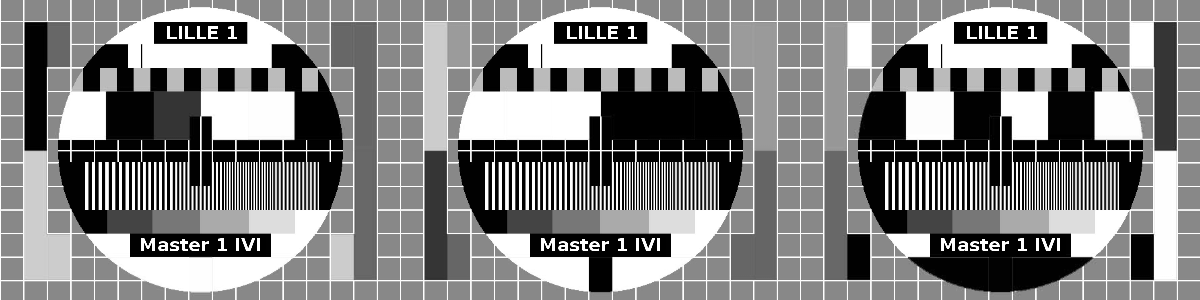
\includegraphics[width=10cm]{../mire_gris.png}
    \caption{Image en niveau de gris}
  \end{figure}
  
  La récupération d'une image dans un dégradé d'une seul couleur, il faut annuler les deux autres canaux en les multipliant par
  zéro.
  
  \begin{figure}[H]
    \center
    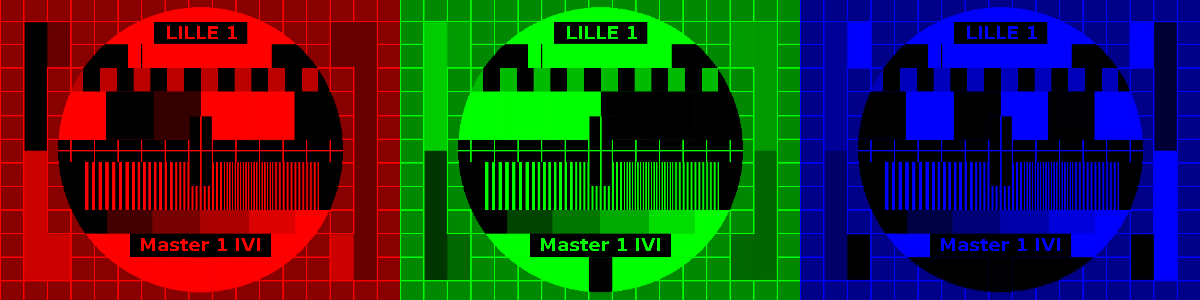
\includegraphics[width=10cm]{../mire_couleur.png}
    \caption{Image avec suppression de deux composantes de couleur}
  \end{figure}
  
  \section{Sur et sous-échantillonnage}
  Nous allons, avant de définir les notions de sur et sous-échantillonage, calculer les dimensions du support
  initial de l'image en prenant comme résolution d'acquisition 72 pixel/pouce. Ce calcul correspond à :
  <nb pixels sur x> / 72 et <nb pixels sur y> /72. Ce qui nous donne un support de 11x8 pouces.
  
  %800/72 = 11
  %600/72 = 8
  \subsection{Sous-échantillonage}
  Pour effectuer un sous-échantillonage, il faut supprimer un pixel tout les N pixels dans le vecteur de chaque canaux.
  Pour cela il faut supprimer une valeur tout les N pixel et supprimer une ligne toutes les N lignes. L'image contiendra
  alors N fois moins de pixels que l'image d'origine et sera donc N fois plus petite. Nous avons alors l'algorithme suivant.\\

  \begin{lstlisting}[caption=Fonction permettant le sous-échantillonnement d'une image]
    function [newImg] = sousEchant(img,n)
        s = size(img);
        newLenX = s(1)/n;
        newLenY = s(2)/n;
        newImg = zeros(newLenX,newLenY);
        for raw=1:newLenY
            for col=1:newLenX
                for c=1:s(3)
                    newImg(col,raw,c) = img(col*n,raw*n,c);
                end;
            end;
        end;
    endfunction;
  \end{lstlisting}
  
  \subsection{Sur-échantillonage}
  Pour le sur-échantillonage, nous avons utilisé le ré-échantillonage au plus proche voisin. Le principe
  est de dupliqué un pixel. Si la valeur de N vaut 2, nous ajoutons un pixel à droite, un en bas et un en diagonale.
  Ce qui nous donne l'algorithme suivant :\\
  
  \begin{lstlisting}[caption=Fonction permettant le sur-échantillonnement d'une image]
    function [newImg] = surEchant(img,n)
    s = size(img);
    lenX = s(1);
    lenY = s(2);
    newImg = zeros(lenX * n,lenY * n, 3);
    for raw=1:lenY
        for col=1:lenX
            for c=1:s(3)
                for i=0:(n-1)
                    for j=0:(n-1)
                        x = ((col*n)-(n-1)) + i;
                        y = ((raw*n)-(n-1)) + j;
                        newImg(x, y, c)
                    end;
                end;
            end;
        end;
    end;
    endfunction;
  \end{lstlisting}
  
  Le problème avec cette algorithme est que l'image va se pixeliser lorsque N va devenir trop grand. Il existe 
  d'autre algorithme de sur-échantillonage mais contrairement à notre algorithme, l'image résultante sera légèrement flouté quand N sera grand.
  La majorité des autres algorithme vont calculer la moyenne dans le voisinage du pixel recherché. Cela a pour 
  effet de créer un dégradé de la couleur autour des pixels connu et donne un rendu flouté.
  
  %\subsection{Cumulation d'échantillonage}
  %TODO faire les tests
  
  \section{Quantification}
  La quantification permet de réduire le nombre de valeur dans un canal afin de minimiser la taille de l'image.\\
  
  Pour trouver la valeur de chaque intervalle, nous avons appliqué la formule suivante : $((maxVal - minVal) / m) / (maxVal - minVal)$
  où m est le nombre d'intervalle souhaité. La valeur de $m$ est égale à $2^{nbBit}$. Par exemple pour 8 bits nous avons 256 
  niveau de gris, donc 256 intervalles.\\
  
  Une fois que nous avons les intervalles, il faut que la valeur de chaque pixel soit égale à la valeur de l'intervalle 
  inférieur à cette valeur. Cette méthode n'est pas la plus optimale mais elle est la plus simple. On pourrait également 
  chercher l'intervalle le plus proche d'un pixel et modifier sa valeur pour qu'il soit égale à la valeur de l'intervalle.
  
  \newpage
  
  %TODO verif algo et test sur image
  \section{Repliement de spectre}
  %question 1 pixel/m -> resPeriode / 150
  Nous allons maintenant calculer la fréquence de l'image suivante :
  \begin{figure}[H]
    \center
    
\includegraphics[width=10cm]{../ti-semaine-3-sinus.png}
    \caption{Motif sinusoïdal}
  \end{figure}
  
  Nous avons d'abord mesuré la période du motif dans l'image en pixels. Nous avons vu que le motif se
  répétait tous les 100 pixels. Nous pouvons déterminer cette période en mètre, en sachant que la résolution
  horizontal est de 150 pixels/pouce, grâce aux calcules : 
  
  $$\frac{100}{150} \simeq 0,66 pouces$$
  $$\frac{0,66}{100} = 0,016896 m$$
  \ \\
  
  Nous avons donc une période de 0,016m pour le motif présent dans l'image.
  Nous pouvons maintenant calculer la fréquence spatial du motif avec le calcule :
  
  $$\frac{1}{0,016896} \simeq 60 cycle/m$$
  $$ = \frac{1}{100} cycle/pixel$$
  
  \newpage
  
  \section*{Conclusion}
  Lors de ce TP, nous avons appris à utiliser des méthode basique de ré-échantillonnement d'image couleur. De plus, 
  nous avons vu que le sous-échantillonage était destructif et qu'il n'était pas possible de récupérer les données
  avec un sur-échantillonage.
 
    
\end{document}  